The three equations that form the model for the segway, namely \autoref{}, \autoref{} and \autoref{} is linearised before they are used in controller design. The reason for this is that the field of designing controllers for linear models are more developed, i.e. a larger variety of methods, which makes the design of controllers easier for linear systems. The model for the motors shown in \autoref{} is already on a linear form, thus only two of the three equations describing the model for the segway is linearised.

When linearising, an operating point is chosen and the linearised model is the tangent to this point. This is shown on \autoref{fig:taylor}. This approach means that the linearised model is only an approximation of the original model around the operating point. During the course Modelling and control, the group was introduced to Taylor expansion as a method to linearise. For this reason the method that will be used to linearise the two model equations is Taylor expansion.

\begin{figure}[H]
\centering
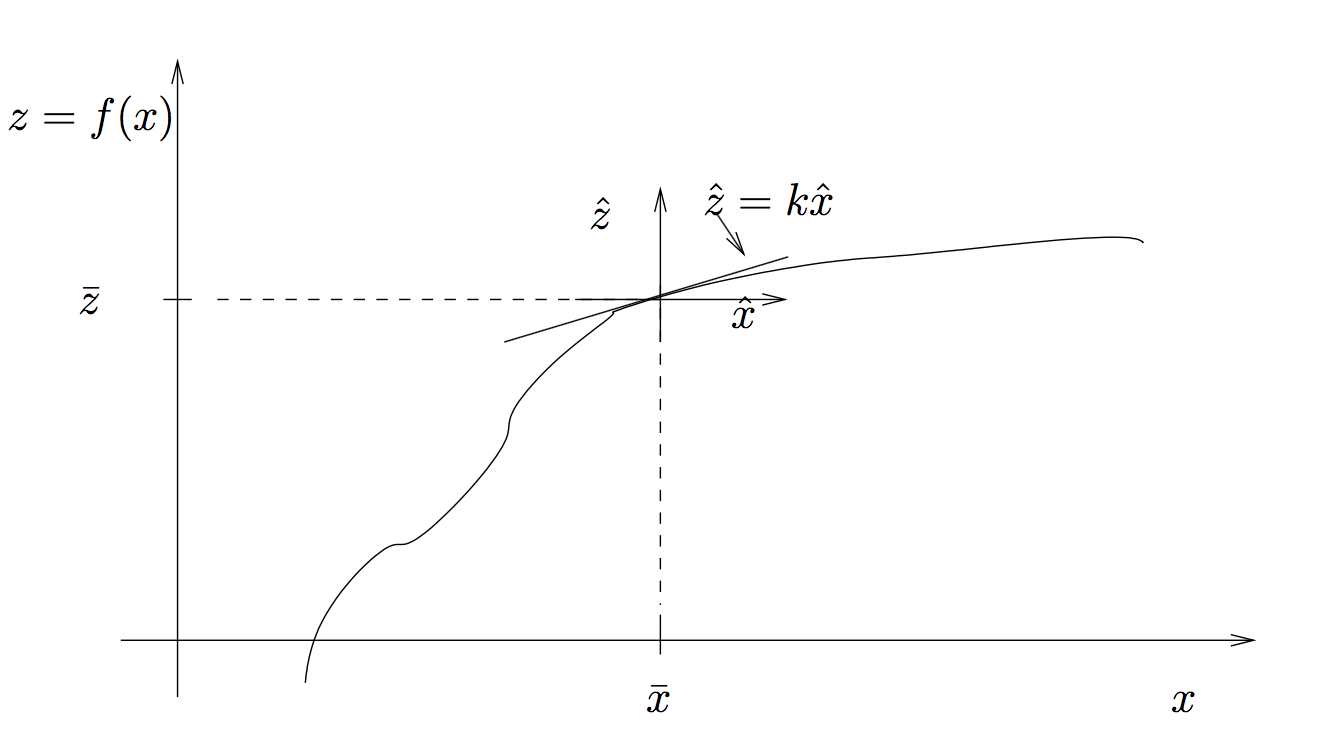
\includegraphics[scale=0.6]{figures/taylor.png}
\caption{Illustration of linearisation principle.}
\label{fig:taylor}
\end{figure}
\todo{Make a new figure}
Taylor expansion is based on the Taylor series, shown in \autoref{eq:taylorSeries}. The Taylor series approximation of an original signal is enhanced by including a greater number of terms in the Taylor series. However, since the linearisation is a tangent, only the first two terms in the Taylor series is used in the Taylor expansion.
\begin{align}
f(x) = f(a) + f'(a)(x - a) + \frac{f''(a)}{2!}(x - a)^2 + \frac{f^{(3)}(a)}{3!}(x - a)^3 + ...
\label{eq:taylorSeries}
\end{align}


The linearisation is performed around the segways upright equilibrium point, where $\theta_p$ equals zero. Taylor expansion therefore introduces an operating point and a linear deviation around it. These can be expressed as follows.
\begin{equation}
\theta_p(t) = \bar{\theta}_p(t) + \hat{\theta}_p(t)
\end{equation}
\begin{where}
\va{$\theta_p(t)$}{is the angle of the pendulum}{rad}\\
\va{$\bar{\theta}_p(t)$}{is the operating point}{rad}\\
\va{$\hat{\theta}_p(t)$}{is the linear deviation}{rad}
\end{where}

As there are up to three variables in the model equations that is to be linearised, i.e. $\theta_p(t)$, $\dot\theta_p(t)$ and $\ddot\theta_p(t)$ the first two terms for the Taylor series for each variable forms the Taylor expansion that can linearise both model equations. The Taylor expansion is shown in \autoref{eq:taylor}.

\begin{align}
P= f(\bar{\theta}_p(t),\bar{\dot \theta}_p(t),\bar{\ddot \theta}_p(t))+ \frac{\partial f}{\partial\theta_p(t)}\cdot \hat{\theta}_p(t)&+\frac{\partial f}{\partial \dot \theta_p(t)}\cdot \hat{\dot \theta}_p(t)+ \frac{\partial f}{\partial \ddot \theta(t)_p}\cdot \hat{\ddot \theta}_p(t)\label{eq:taylor}
\end{align}
\begin{where}
\va{$P$}{is the taylor approximation}{1}\\
\end{where}
\todo{representation of formular, supervisor not agreeing with the way it is written, Ralf has made changes to this formular, and now believes it is right.}


The two model equations are shown in \autoref{eq:firstModel} and \autoref{eq:secondModel}, where each term that will be linearised by applying the Taylor expansion, shown in \autoref{eq:taylor}, is marked. 

\begin{align*}
\underbrace{(J_p + m_p \cdot l^2)(m_p + m_c)\ddot \theta_p(t)\rule[-12pt]{0pt}{5pt}}_{\mbox{1}}
\end{align*}
\vspace{-1.1 cm}
\begin{align*}
\\
=
\\
\end{align*}
\vspace{-1.1 cm}
\begin{align}
\underbrace{(m_p^2 + m_c \cdot m_p)l \cdot g \cdot sin(\theta_p(t))\rule[-12pt]{0pt}{5pt}}_{\mbox{2}} + \underbrace{m_p^2 \cdot l^2 \cdot cos^2(\theta_p(t)) \cdot \ddot \theta_p(t)\rule[-12pt]{0pt}{5pt}}_{\mbox{3}} - \underbrace{m_p \cdot l \cdot \dot \theta_p(t)^2 \cdot sin(\theta_p(t))\rule[-12pt]{0pt}{5pt}}_{\mbox{4}} + 2 \cdot F_F(\theta_p(t))
\label{eq:firstModel}
\end{align}

\begin{align}
\ddot \theta_m(t) = \underbrace{\frac{(J_p + m_p\cdot l^2)\ddot \theta_p(t)}{m_p \cdot l \cdot \cos(\theta_p(t))\cdot r_w \cdot N_{ms} \cdot N_{sw}}\rule[-12pt]{0pt}{5pt}}_{\mbox{1}} - \underbrace{\frac{g \cdot sin(\theta_p(t)}{cos(\theta_p(t))\cdot r_w \cdot N_{ms} \cdot N_{sw}}\rule[-12pt]{0pt}{5pt}}_{\mbox{2}}
\label{eq:secondModel}
\end{align}

The result of the linearisations are shown in \autoref{eq:firstModelLin} and \autoref{eq:secondModelLin}, and the deriviation of these results can be found in \autoref{app:firstModel} and \autoref{app:secondModel}.
\begin{align}
\underbrace{(J_p + m_p \cdot l^2)(m_p + m_c) \cdot \hat{\ddot \theta}_p(t)\rule[-12pt]{0pt}{5pt}}_{\mbox{1}} = \underbrace{(m_p^2 + m_c \cdot m_p)l \cdot g \cdot \hat{\theta}_p(t)\rule[-12pt]{0pt}{5pt}}_{\mbox{2}} + \underbrace{m_p^2 \cdot l^2 \cdot \hat{\ddot \theta}_p(t)\rule[-12pt]{0pt}{5pt}}_{\mbox{3}} + 2 \cdot F_F(\theta(t))
\label{eq:firstModelLin}
\end{align}

\begin{align}
\ddot \theta_m(t) = \underbrace{\frac{(J_p + m_p \cdot l^2)}{m_p \cdot l \cdot r_w \cdot N_{ms} \cdot N_{sw}}\hat{\ddot \theta}_p(t)\rule[-12pt]{0pt}{5pt}}_{\mbox{1}} - \underbrace{\frac{g}{r_w \cdot N_{ms} \cdot N_{sw}} \hat{\theta}_p(t)\rule[-12pt]{0pt}{5pt}}_{\mbox{2}}
\label{eq:secondModelLin}
\end{align}

\subsection{Laplace Transform}
From the previous sections tree expressions have been derived. One for the motor model and one for the pendulum model. Moreover an expression, which is the link between the two models, is found. 
The motor model is the following:
\begin{equation}
\tau_a(t) = \frac{k_t}{R_A} \left( V_a(t) - K_e \cdot \dot\theta_m(t) \right) - \ddot\theta_m(t)J_{T} - \dot\theta_m(t)B_{T}  \label{eq:motorfinal2}
\end{equation}
Laplace transforming \autoref{eq:motorfinal2} yields:
\begin{align}
\tau_a(s)&=\frac{k_t}{R_A}- \Theta_m(s) (s\cdot \frac{k_t+k_e}{R_a}+s\cdot B_T+s^2\cdot J_T)\\
&=\frac{k_t}{R_A}- \Theta_m(s)(s^2\cdot J_T+s(\frac{k_t+k_e}{R_a}+B_T))
\end{align}
The link between the two models shall be laplace transformed as well. The link in time domain is:
\begin{align}
 \hat{\ddot\theta}_m(t)=\frac{(J_p+m_p\cdot l^2)\hat{\ddot \theta}_p(t)}{m_p\cdot l\cdot r_w\cdot N_{ms}\cdot N_{sw}}-\frac{g\cdot \hat{\theta}_p(t)}{r_w\cdot N_{ms}\cdot N_{sw}}\label{eq:linktime}
\end{align}
Laplace transforming \autoref{eq:linktime} yields:
\begin{align}
s^2\cdot \Theta_m(s)&= \frac{(J_p+m_p\cdot l^2)s^2\cdot \Theta_p(s)}{m_p\cdot l \cdot r_w \cdot N_{ms}\cdot N_{sw}}-\frac{g\cdot \Theta_p(s)}{r_w\cdot N_{ms}\cdot N_{sw}}\\
\Rightarrow \Theta_m(s)&= \frac{(J_p+m_p\cdot l^2)\Theta_p(s)}{m_p\cdot l \cdot r_w \cdot N_{ms}\cdot N_{sw}}-\frac{g\cdot \Theta_p(s)}{s^2 \cdot r_w\cdot N_{ms}\cdot N_{sw}}
\end{align}
Lastly the model for the pendulum. The model expression is: 
\begin{equation}
(J_p+m_p\cdot l^2)\hat{\ddot \theta}_p(t)(m_p+m_c)=(m_p^2+m_c)l\cdot g \cdot \hat{\theta}_p(t)+m_p^2\cdot l^2 \cdot  \hat{\ddot\theta}_p(t)+2\cdot F_F(\theta_p(t))\label{eq:penmodel11}
\end{equation}
Laplace transforming \autoref{eq:penmodel11} yields:
\begin{equation}
s^2(J_p+m_p\cdot l^2)\Theta_p(s)(m_p+m_c)=(m_p^2+m_c)l\cdot g \cdot \Theta_p(s) + m_p^2 \cdot l^2 \cdot s^2\cdot \Theta_p(s) +2\cdot F_F(\Theta_p(s))
\end{equation}
As the input to pendulum from the motors are the applied force, it is preferable to have this linearized model as an expression of the applied force. 
\begin{equation}
2\cdot F_F(\Theta_p(s))=\Theta_p(s)(s^2((J_p+m_p\cdot l^2)(m_p+m_c)-m_p^2\cdot l^2)-(m_p^2 + m_c)l\cdot g)
\end{equation}

%
%\begin{align}
%&s^2\cdot \theta\cdot (l\cdot (m_p+m_c-m_p))-\theta \cdot g(m_p+m_c)=F_F\nonumber\\
%&\Rightarrow \frac{\theta}{F_F}=\frac{1}{s^2\cdot (l\cdot (m_p+m_c)-g(m_p+m_c)}\nonumber \\
%&\Rightarrow \frac{\frac{1}{l\cdot m_c}}{s^2-\frac{g(m_p+m_c}{l\cdot m_c}}
%\end{align}
%It shows, that the transfer function is the same as the one derived at with the taylor expansion approximation. \\
%The linear approximation of the inverted pendulum model is therefore assumed valid. 
%
%
%
%%\Rightarrow\frac{2.377}{s^2 - 37.369}
%%\Rightarrow \theta(s)\cdot s^2\cdot l ((m_p+m_c)-m_p)=g\cdot \theta(s)\cdot (m_p+m_c)+F_F(s)\nonumber\\
%%\Rightarrow \theta(s)\cdot s^2\cdot l(m_p+m_c-m_p)-g\cdot \theta(s)\cdot(m_p+m_c)=F_F(t)\nonumber\\
%%\Rightarrow \theta(s)\cdot (s^2\cdot l \cdot (m_p+m_c))=F_F(t) \nonumber \\
%The transfer function for the inverted pendulum shall be merged with a transfer function for the motors and wheels model to allow design and implementation of a controller. Merging the transfer functions is done in the following section. 
